\documentclass[10pt,letterpaper]{article}
\usepackage{mathpazo}
\usepackage[scaled]{helvet}
\usepackage[T1]{fontenc}
\usepackage{hyperref}
\usepackage{color,soul}
\usepackage{graphicx}
\usepackage[justification=centering,singlelinecheck=false]{caption}
%\usepackage{setspace}
\usepackage[margin=1in,includehead,includefoot]{geometry}
\usepackage[table,dvipsnames]{xcolor}
\usepackage{amssymb}
\usepackage{amsmath}
\usepackage{fancyhdr}
\usepackage{array}
\usepackage{gensymb}
\usepackage{lastpage}
\usepackage{textcomp}
\usepackage{booktabs}
\usepackage{pdfpages}
\usepackage{tabto}
\usepackage{multicol}
\usepackage{tabularx}
\usepackage{framed}
\usepackage{chngcntr}
\usepackage{tocloft}
\usepackage[font={sf,normalsize},labelfont={sf,bf}]{caption}
\usepackage{float}
\usepackage{tikz}
\usepackage{listings}
\lstset{basicstyle=\small\ttfamily,breaklines=true}
\usepackage{forest}
\usepackage{verbatim}
\usepackage{longtable}
\usepackage{tabu}
\usepackage{afterpage}
\usepackage{paralist}
\usepackage{indentfirst}
\usepackage{changepage}

\newenvironment{Figure}
{\par\medskip\noindent\minipage{\linewidth}}
{\endminipage\par\medskip}

%% no indentation
%\setlength{\parindent}{0pt}

%%header and footer
\fancyhf{}
\renewcommand{\footrulewidth}{0pt}
\renewcommand{\headrulewidth}{0pt}
\rhead{\nouppercase{\leftmark}}
\lhead{\sf \textbf{Project 2}  |  Reinforcement Learning}
\rfoot{\sf \textbf{0\thepage} OF \textbf{0\pageref*{LastPage}}}
\rhead{\sf \textbf{AA 228} | Decision Making Under Uncertainty}
\pagestyle{fancy}


%% DOCUMENT START --------------------------------------------------

\begin{document}
		
	\captionsetup[figure]{labelformat=simple, labelsep=quad, labelfont={sf, bf}}
	\captionsetup[table]{labelformat=simple, labelsep=quad, labelfont={sf, bf}}
	
	\section*{\sf \textbf{Reinforcement Learning}}
	\vspace*{-0.1 in}
	{\noindent \sf \large R. B. Alexander}
	
	\vspace*{0.2 in}
	
\begin{adjustwidth}{1cm}{1cm}
		
	\noindent \textbf{Reinforcement learning (RL) is a technique for training an agent in an environment to take actions that maximize the expected utility over a given horizon - solving a Markov decision process (MDP). We focus here on infinite horizon problems with discount factor $\boldsymbol\gamma$. At time $\boldsymbol t$, the agent is in state $\boldsymbol{s_t} \boldsymbol{\in} \boldsymbol{\mathcal{S}}$ and can take action $\boldsymbol{a_t} \boldsymbol{\in} \boldsymbol{\mathcal{A}}$. Using the value function $\boldsymbol{U(s)}$ or the state-action value function $\boldsymbol{Q(s,a)}$ (or an approximation thereof), which describes the discounted future expected utility of being in state $\boldsymbol s$ and taking action $\boldsymbol a$, the agent selects the optimal action according to the optimal policy $\boldsymbol{a_t} = \boldsymbol{\pi^*(s_t)}$. The agent takes action $\boldsymbol a_t$, receives reward $\boldsymbol r_t$, and transitions to state $\boldsymbol{ s_{t+1}}$. Under the Markov assumption, the state transition model $\boldsymbol{T(s_{t+1}} \boldsymbol{\mid} \boldsymbol{s_t}, \boldsymbol{a_t})$ and reward model $\boldsymbol{R(s_t,a_t)}$ are stationary. Various techniques can be used to compute optimal or approximately optimal policies for acting in the environment. When the transition model and reward model are known exactly, an optimal policy can be computed using dynamic programming algorithms (value iteration, policy iteration, direct policy search); when the transition model and reward model are not known exactly, an approximately optimal policy can be computed using approximate dynamic programming algorithms (maximum-likelihood estimation of $\boldsymbol T$ and $\boldsymbol R$, Q-learning, SARSA, local approximation, global approximation). In the following paper, we utilize these algorithms, discuss and utilize methods for improving generalization, and show results for three datasets of varying size that have discretized state and action spaces.}
	
\end{adjustwidth}
		
		\vspace*{0.05 in}
		
\begin{multicols*}{2}
					
	\subsection*{\sf \textbf{Modifications for Improving Generalization}}
	
	Among the challenges present in reinforcement learning -- assigning credit to past actions, generalizing from limited experience, and balancing exploration and exploitation -- generalization is arguably the most difficult. We present methods below that we used in improving generalization of the policies found using general RL algorithms.
		
	\subsubsection*{\sf \textbf{Modal Policy Updating}}
	
	We introduce modal policy updating as a way of locally generalizing from limited experience. The principle is that the policies in the neighborhood of an unvisited state are a good approximation for the policy of the unvisited state. The policy of the unvisited state is the most likely policy of the neighborhood, so we use the mode of the neighborhood's policy. A suitable representation for the neighborhood of $s$ used herein is that the $\ell_1$ norm of two state representations should be less than some distance $r$. It is appropriate to normalize the components of the state representation relative to the size of the state space along each dimension. For example, suppose we have a state space $\mathcal{S}$ with 50,000 states that can be decomposed into a representation in $s_1 \times s_2 \subset \mathbb{Z}^2 $ with $s_1 = [1,100], s_2 = [1, 500]$. A suitable condition for the neighborhood around $s'$ could be the following condition.
	 
	$$(s_1-s')^2 + \left(\frac{s_2-s'}{5}\right)^2 \leq R^2$$ 
	
	For modal policy updating, we first compute the value function and optimal policy for the discretized state space using any algorithm without generalization techniques (value iteration, policy iteration, policy search, Q-learning, Sarsa, eligibility trace methods) and make a copy of the optimal policy called $\tilde\pi$. Then for each state in $\mathcal{S}$, we follow the following procedure. First, compute the neighborhood of $s$, $N(s) \subset \mathcal{S}$, where the neighborhood excludes $s$. The structure of the state space can be exploited to define an efficient neighborhood representation. Then, remove the states in the neighborhood where the value function at $s$ is 0 to select the valid neighborhood $N'(s) = {s \in N(s) | U(s) \ne 0}$. If the valid neighborhood is non-empty, the policy at $s$, updated to the mode of the policies of the valid neighborhood $\tilde\pi(s) = mode(\pi(N'(s)))$. After iterating over the state space, the modally-updated policy is $\tilde\pi$.
	
	
	\subsubsection*{\sf \textbf{Global Approximation using Fourier Series Expansion}}
	
	Global approximation is used to approximate the value function over the entire state space. Since the Fourier series can approximate any function, we use a several-term decomposition to approximate the value function without resorting to arbitrary basis functions. Using an efficient representation of the state space leads to better approximation. In the cases presented here, the most efficient representation was 2D, so a 2D Fourier series expansion $f_a(s_1, s_2)$ with lengthscales $\lambda_{s_1}, \lambda_{s_2}$ was used with three terms and decomposed along the action space for $a \in \mathcal{A}$:
	\begin{align*}
	f_a(s_1, s_2) & = \sum_{n=1}^{3}\sum_{m=1}^{3}\alpha_{n,m}\cos\left(\frac{2\pi n s_1}{\lambda_{s_1}}\right)\cos\left(\frac{2\pi m s_2}{\lambda_{s_2}}\right) \\
	& + \sum_{n=1}^{3}\sum_{m=1}^{3}\beta_{n,m}\cos\left(\frac{2\pi n s_1}{\lambda_{s_1}}\right)\sin\left(\frac{2\pi m s_2}{\lambda_{s_2}}\right) \\
	& + \sum_{n=1}^{3}\sum_{m=1}^{3}\gamma_{n,m}\sin\left(\frac{2\pi n s_1}{\lambda_{s_1}}\right)\cos\left(\frac{2\pi m s_2}{\lambda_{s_2}}\right) \\
	& + \sum_{n=1}^{3}\sum_{m=1}^{3}\delta_{n,m}\sin\left(\frac{2\pi n s_1}{\lambda_{s_1}}\right)\sin\left(\frac{2\pi m s_2}{\lambda_{s_2}}\right) \\
	& + c
	\end{align*}
	
	\subsection*{\sf \textbf{Results}}
	
	In our implementation, we used a variety of methods including:
	\begin{compactenum}
		\item value iteration using the maximum-likelihood estimate of $T$ and $R$
		\item Gauss-Seidel value iteration using the maximum-likelihood estimate of $T$ and $R$
		\item sarsa($\lambda$)
		\item sarsa($\lambda$) with local approximation (k-nearest neighbors)
		\item sarsa($\lambda$) with global approximation (fourier series)
	\end{compactenum}
	For each of the above, we performed modal policy updating.
	
	\subsubsection*{\sf \textbf{Small Dataset}}
	
	The \texttt{small} dataset describes a 10x10 grid-world with $|\mathcal{S}| = 100$ and $|\mathcal{A}| = 4$. The discount factor for the problem is given to be $\gamma = 0.95$. The dataset has a convenient representation as two position $(x,y)$ coordinates in space and the actions represent moving left, right, up, or down. For this dataset, we show the results of Gauss-Seidel value iteration and sarsa($\lambda$) with global approximation. Value iteration performs best here, even with the tuning of the learning rate and eligibility trace parameter for sarsa. We observe the convergence of the Fourier series to an approximate value function, though it does not yield as good of a policy as value iteration.
	
	Since the state space was relatively small and most states had a nonzero value function, the modally-updated policies are essentially equivalent to the original policies.
	
	\begin{Figure}
		\centering
		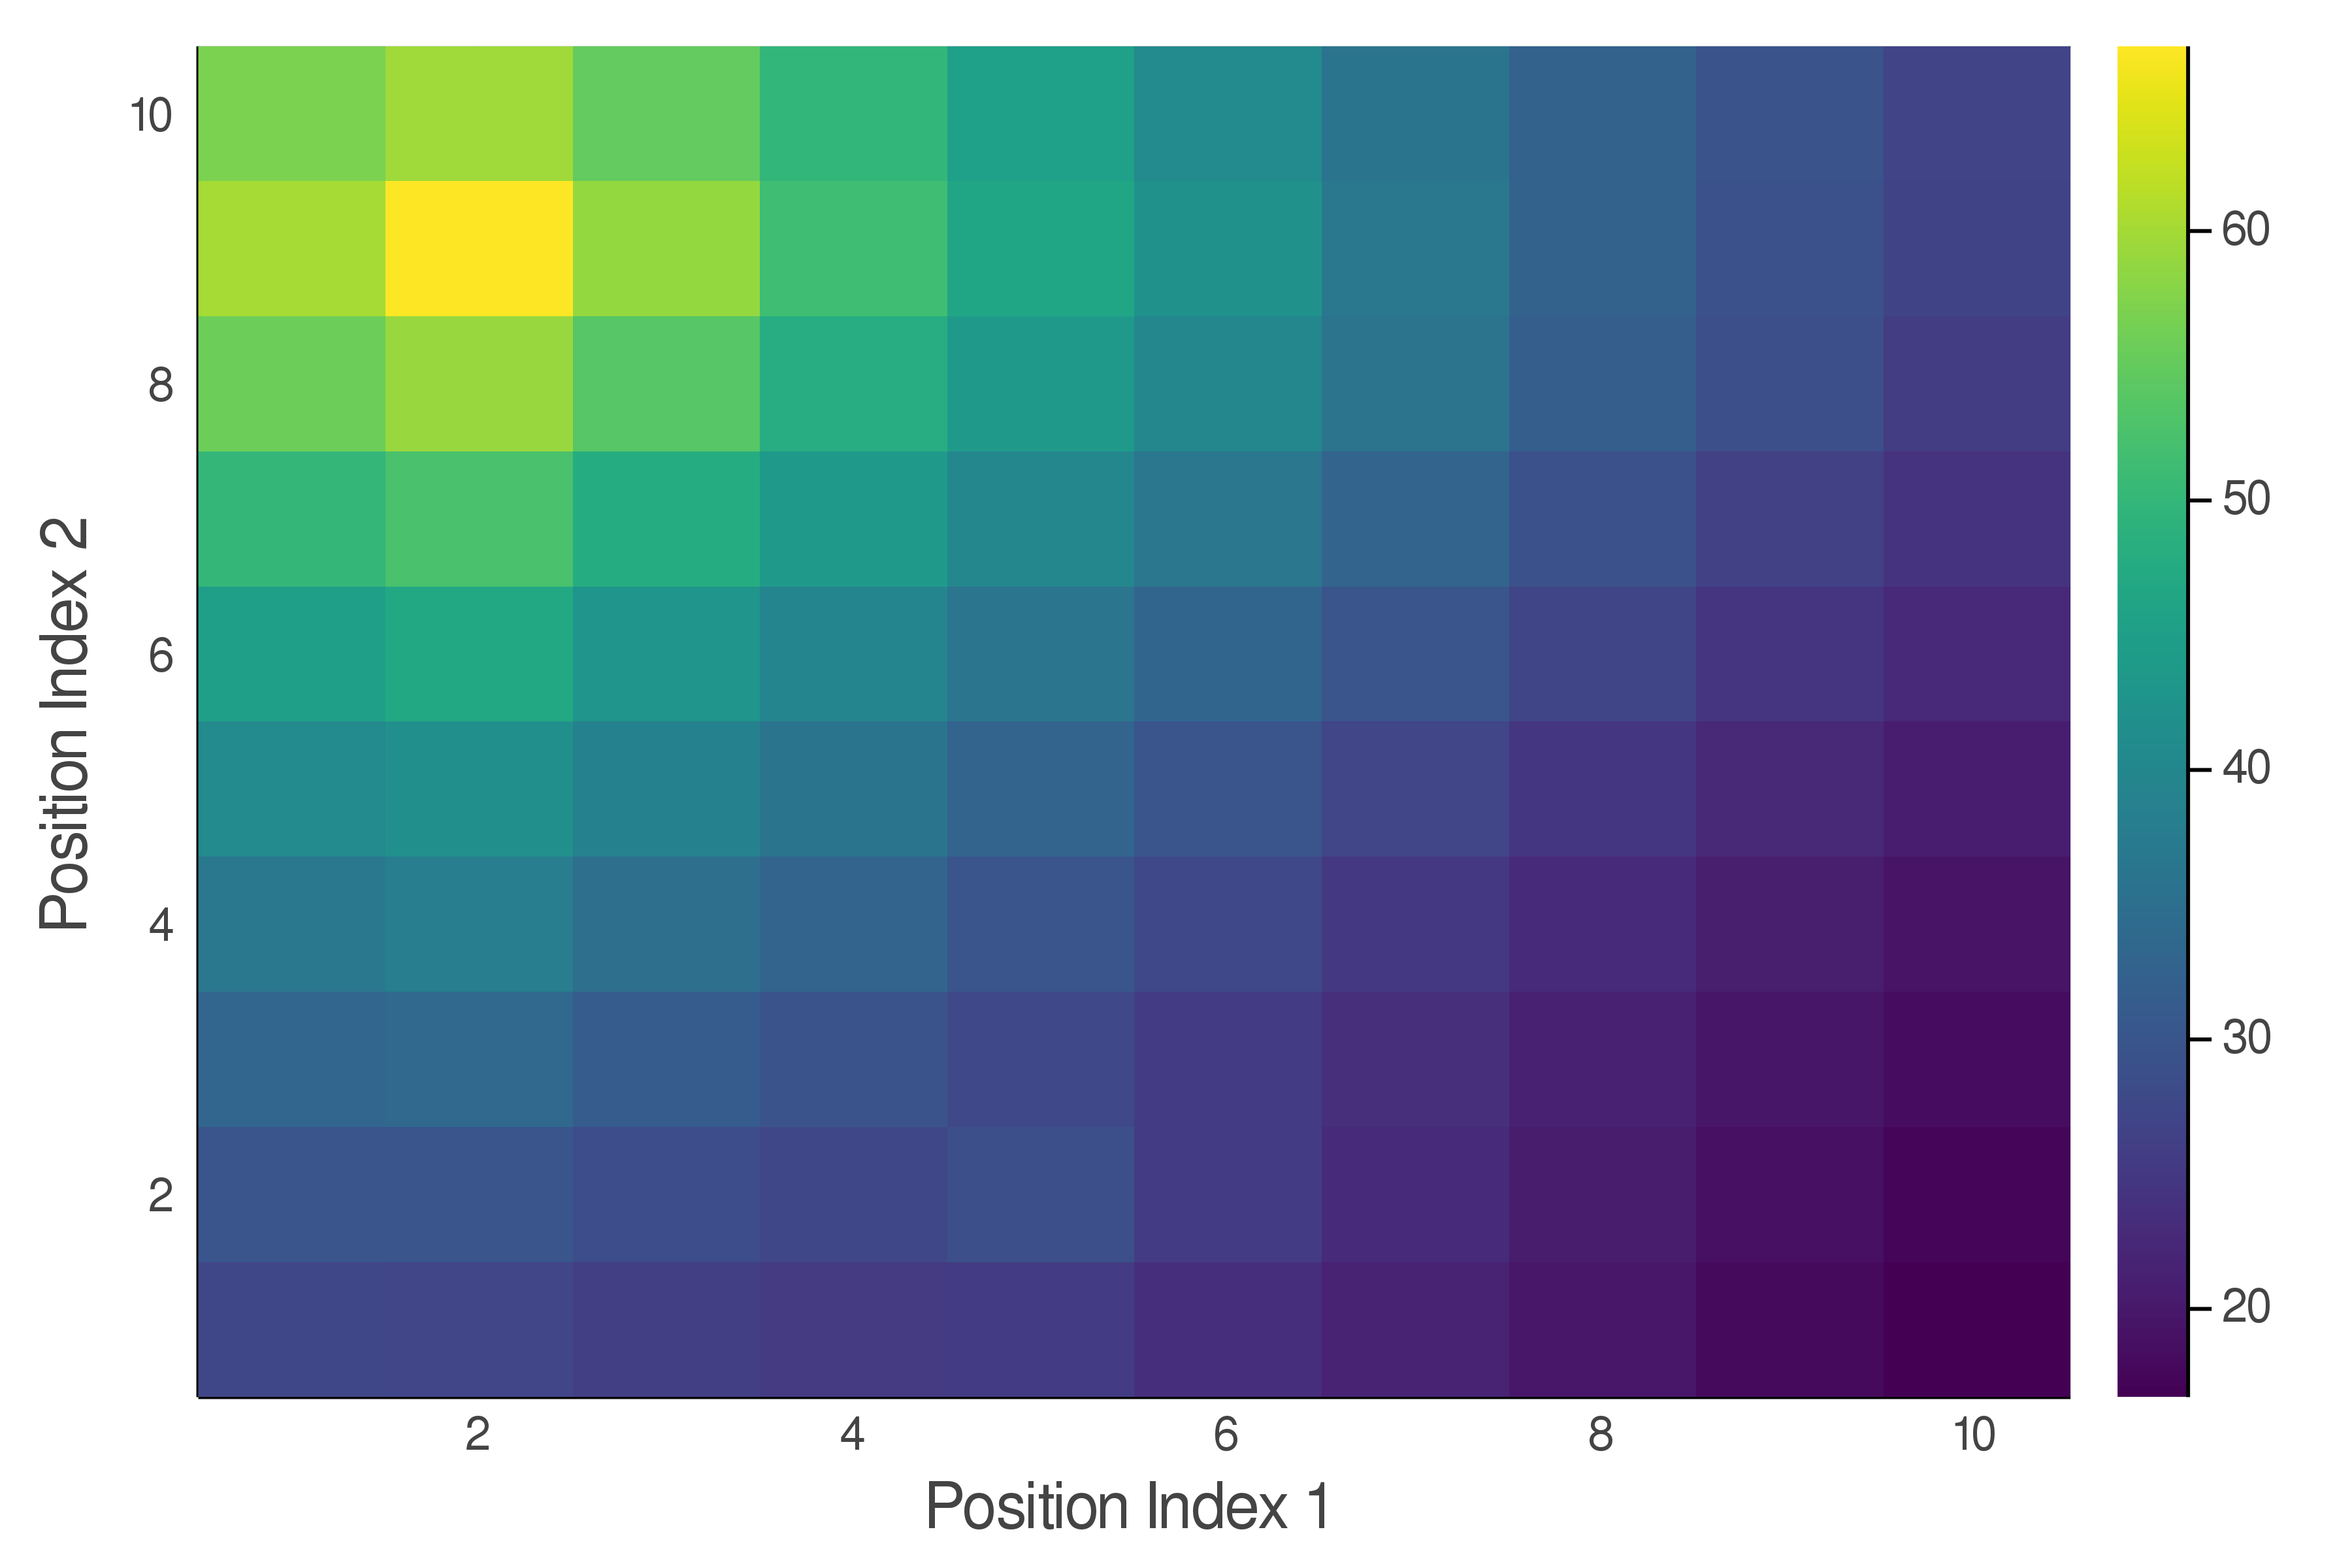
\includegraphics[width=\linewidth]{../plots/small_U_GSVI.png}
		\includegraphics[width=\linewidth]{../plots/small_π_GSVI.png}
		\captionof{figure}{Optimal value function and policy in the positional state space representation using Gauss-Seidel value iteration ($\epsilon = 0.1$) for the \texttt{small} dataset.}
		\label{fig:small_U_GSVI}
	\end{Figure}
	\begin{Figure}
		\centering
		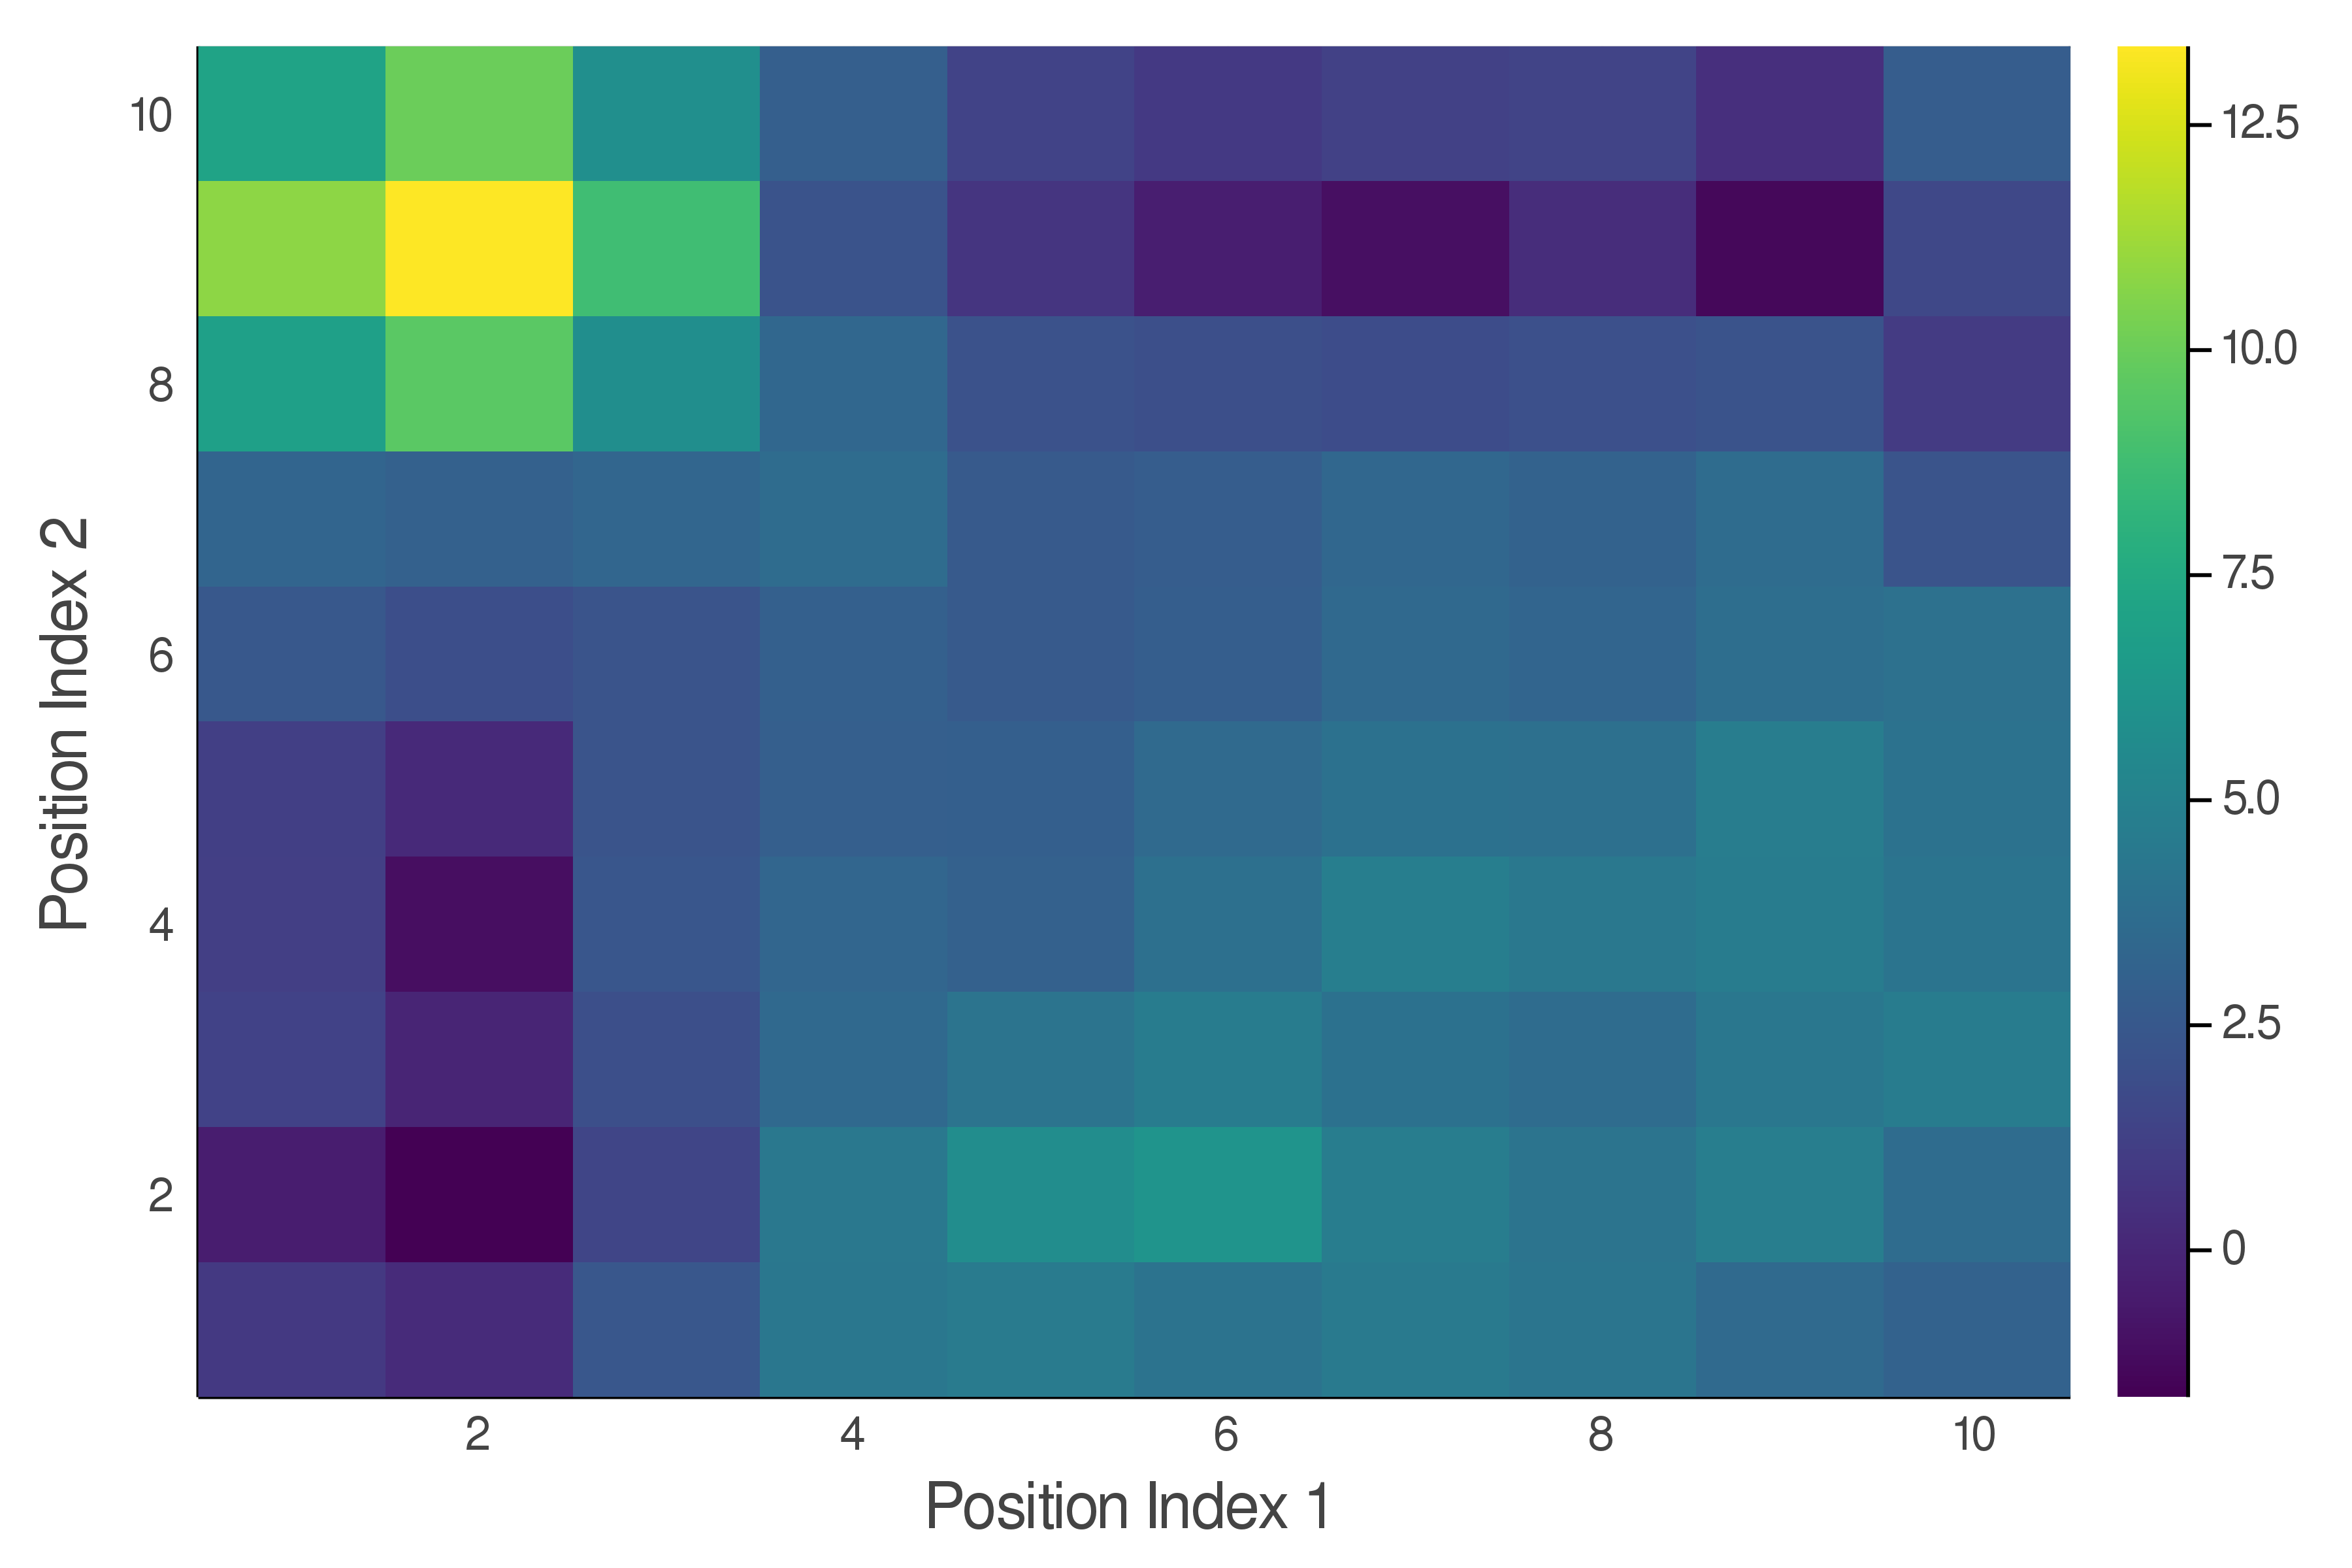
\includegraphics[width=\linewidth]{../plots/small_U_sarsaLambdaGA.png}
		\includegraphics[width=\linewidth]{../plots/small_π_sarsaLambdaGA.png}
		\captionof{figure}{Optimal value function and policy in the positional state space representation using sarsa($\lambda$) with global approximation ($\lambda = 0.9; \alpha = 0.05$) for the \texttt{small} dataset.}
		\label{fig:small_U_slga}
	\end{Figure} \vspace*{-0.3 in}	
	
	\subsubsection*{\sf \textbf{Medium Dataset}}
	
	The \texttt{medium} dataset describes mountain car environment with $|\mathcal{S}| = 50000$ and $|\mathcal{A}| = 7$. The problem is given to be undiscounted. The dataset has a convenient representation as position and velocity $(x,v)$ coordinates in phase space and the actions represent varying degrees of positive and negative acceleration. For this dataset, we performed Gauss-Seidel value iteration and sarsa($\lambda$). Value iteration performs best for the cost and ease of use. Since the state space is relatively large and we have many missing states in our dataset, the modally-updated policies are even better than the original policies, which are missing reasonable policies for the unvisited states. Our condition for the neighborhood was: $(v-v')^2 + ((x-x')/5)^2 \leq (1.5)^2$.
	\begin{Figure}
		\centering
		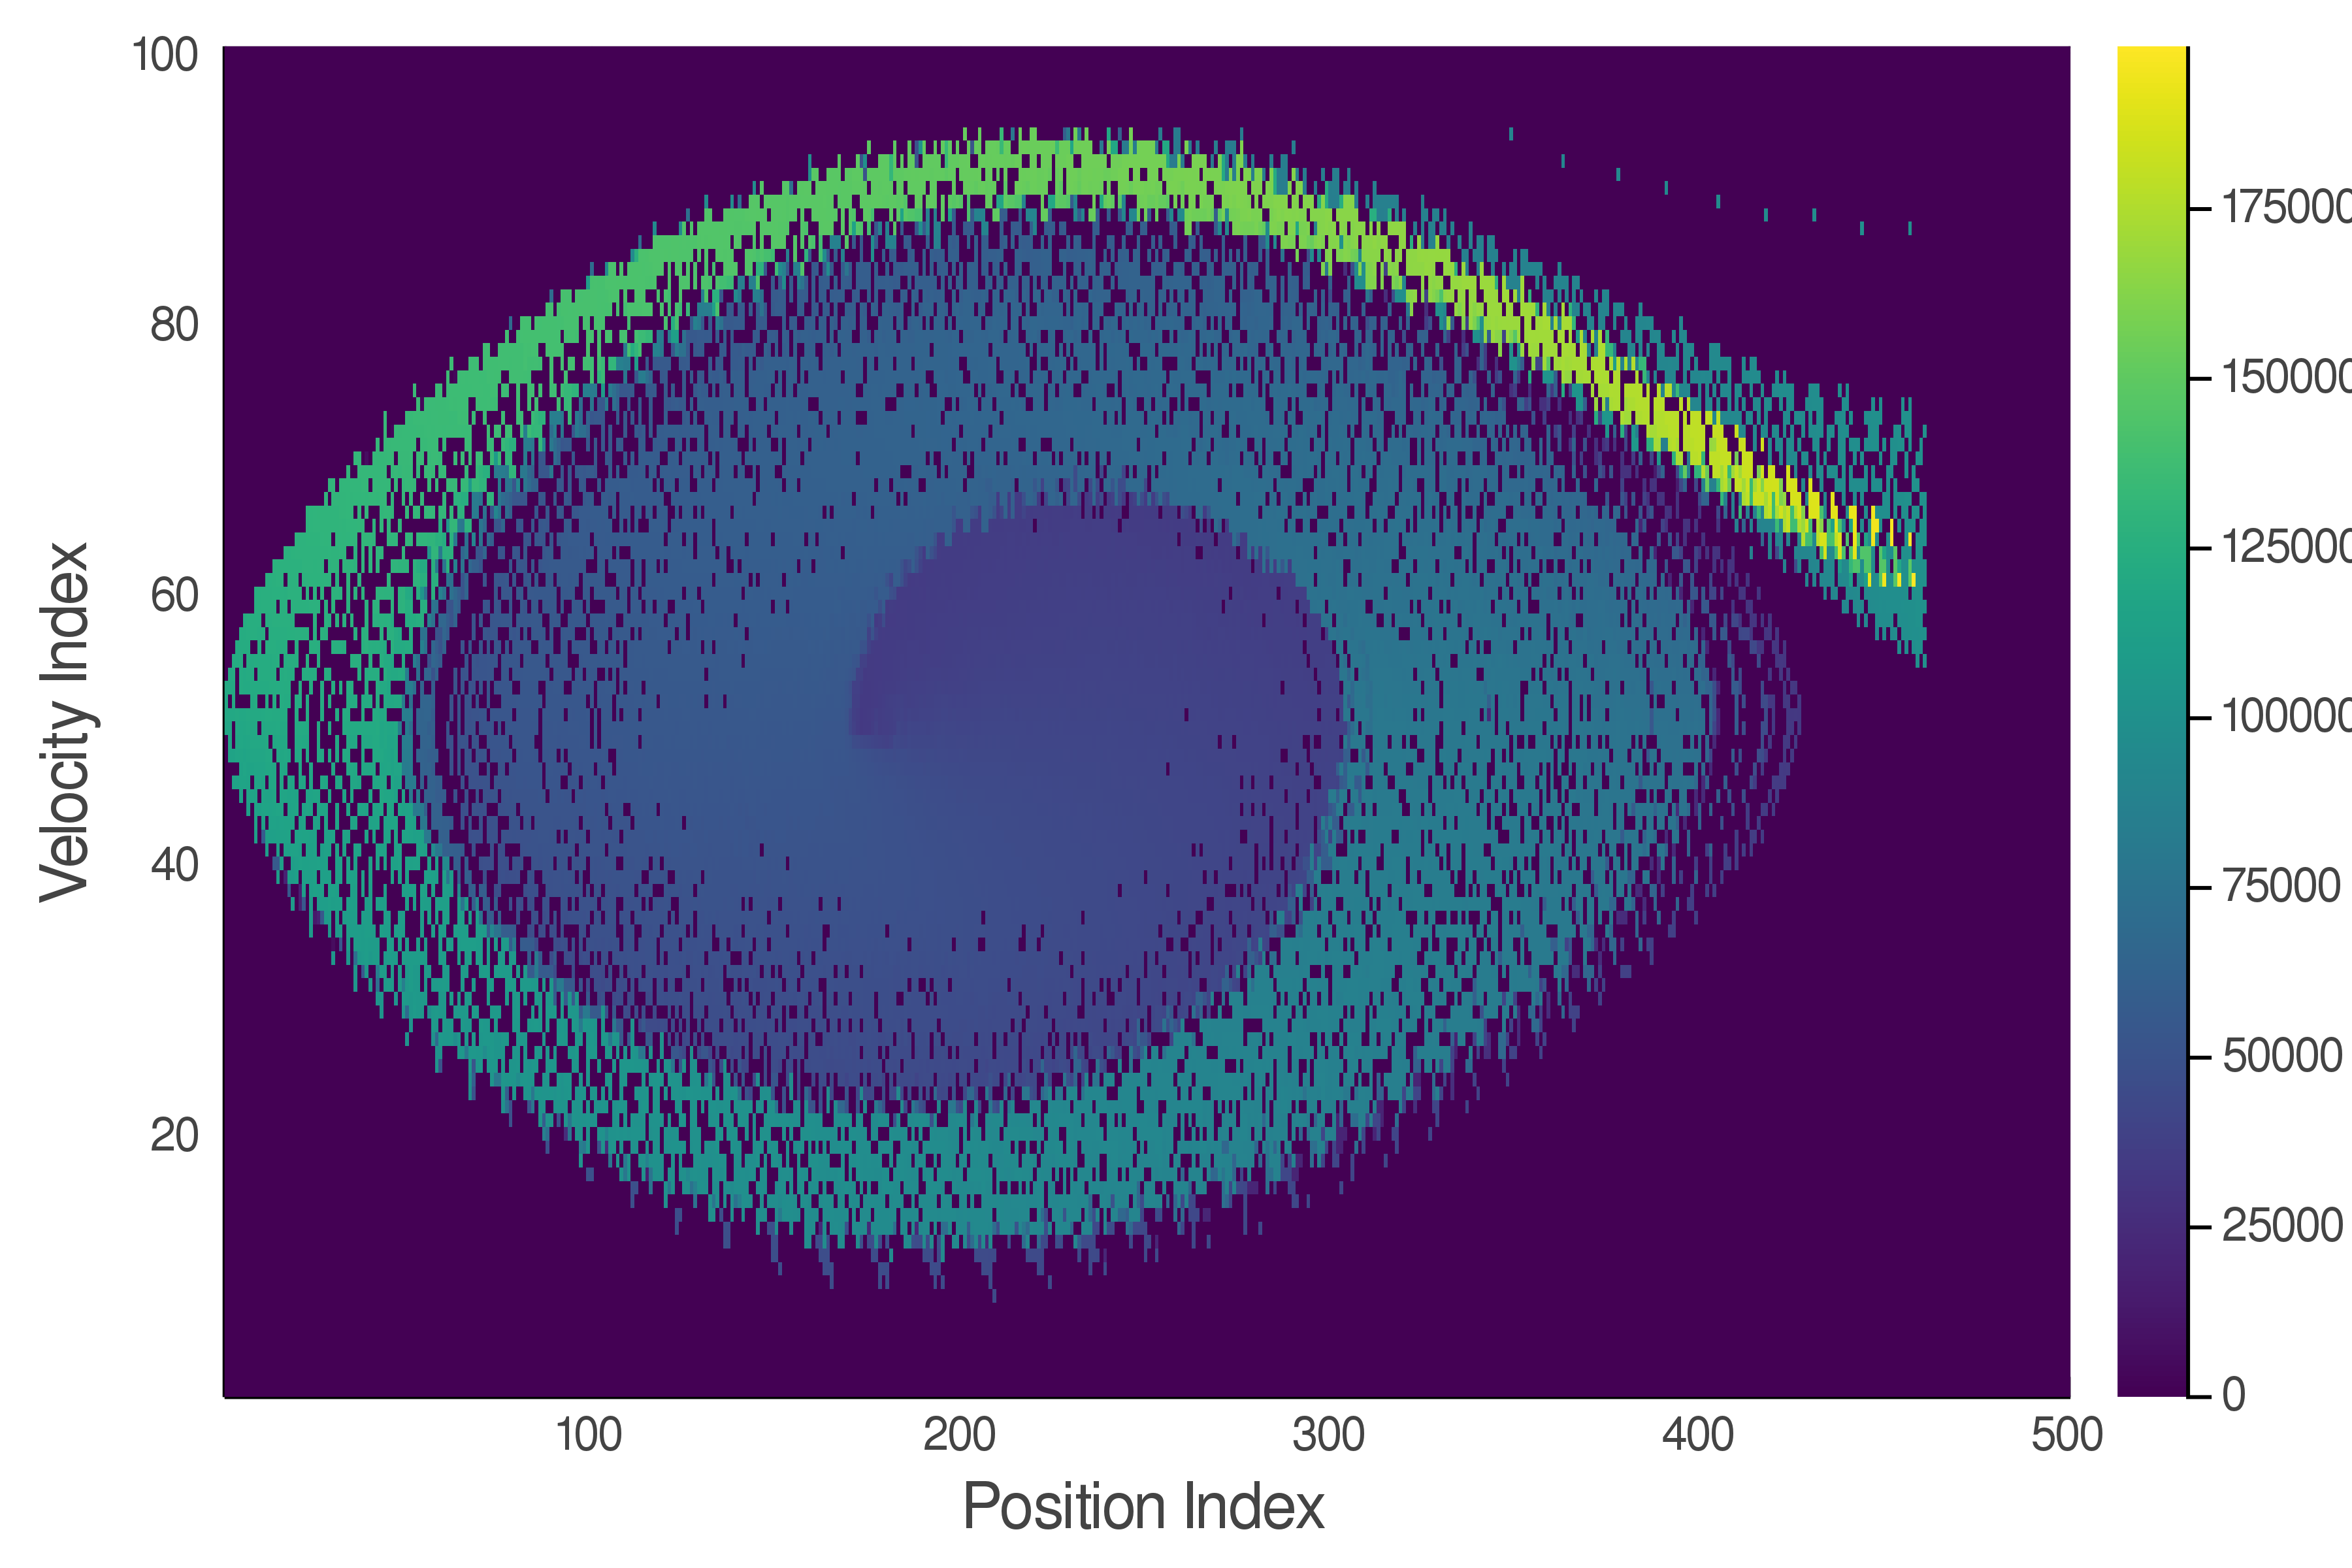
\includegraphics[width=\linewidth]{../plots/medium_U_GSVI.png}
		\includegraphics[width=\linewidth]{../plots/medium_π_GSVI.png}
		\captionof{figure}{Optimal value function and policy in the phase space representation using Gauss-Seidel value iteration ($\gamma = 0.99; \epsilon = 1000$) for the \texttt{medium} dataset.}
		\label{fig:medium_U_GSVI}
	\end{Figure}
	\begin{Figure}
		\centering
		\includegraphics[width=\linewidth]{../plots/medium_πModal_GSVI.png}
		\captionof{figure}{Optimal modally-updated policy in the phase space representation using Gauss-Seidel value iteration ($\gamma = 0.99; \epsilon = 1000$) for the \texttt{medium} dataset.}
		\label{fig:medium_πm_GSVI}
	\end{Figure}
	Sarsa runs can give good policies but at the expense of having to tuning the learning rate and eligibility trace parameter and re-run the algorithm. As a result, we did not find a decent policy using sarsa. 
	\begin{Figure}
		\centering
		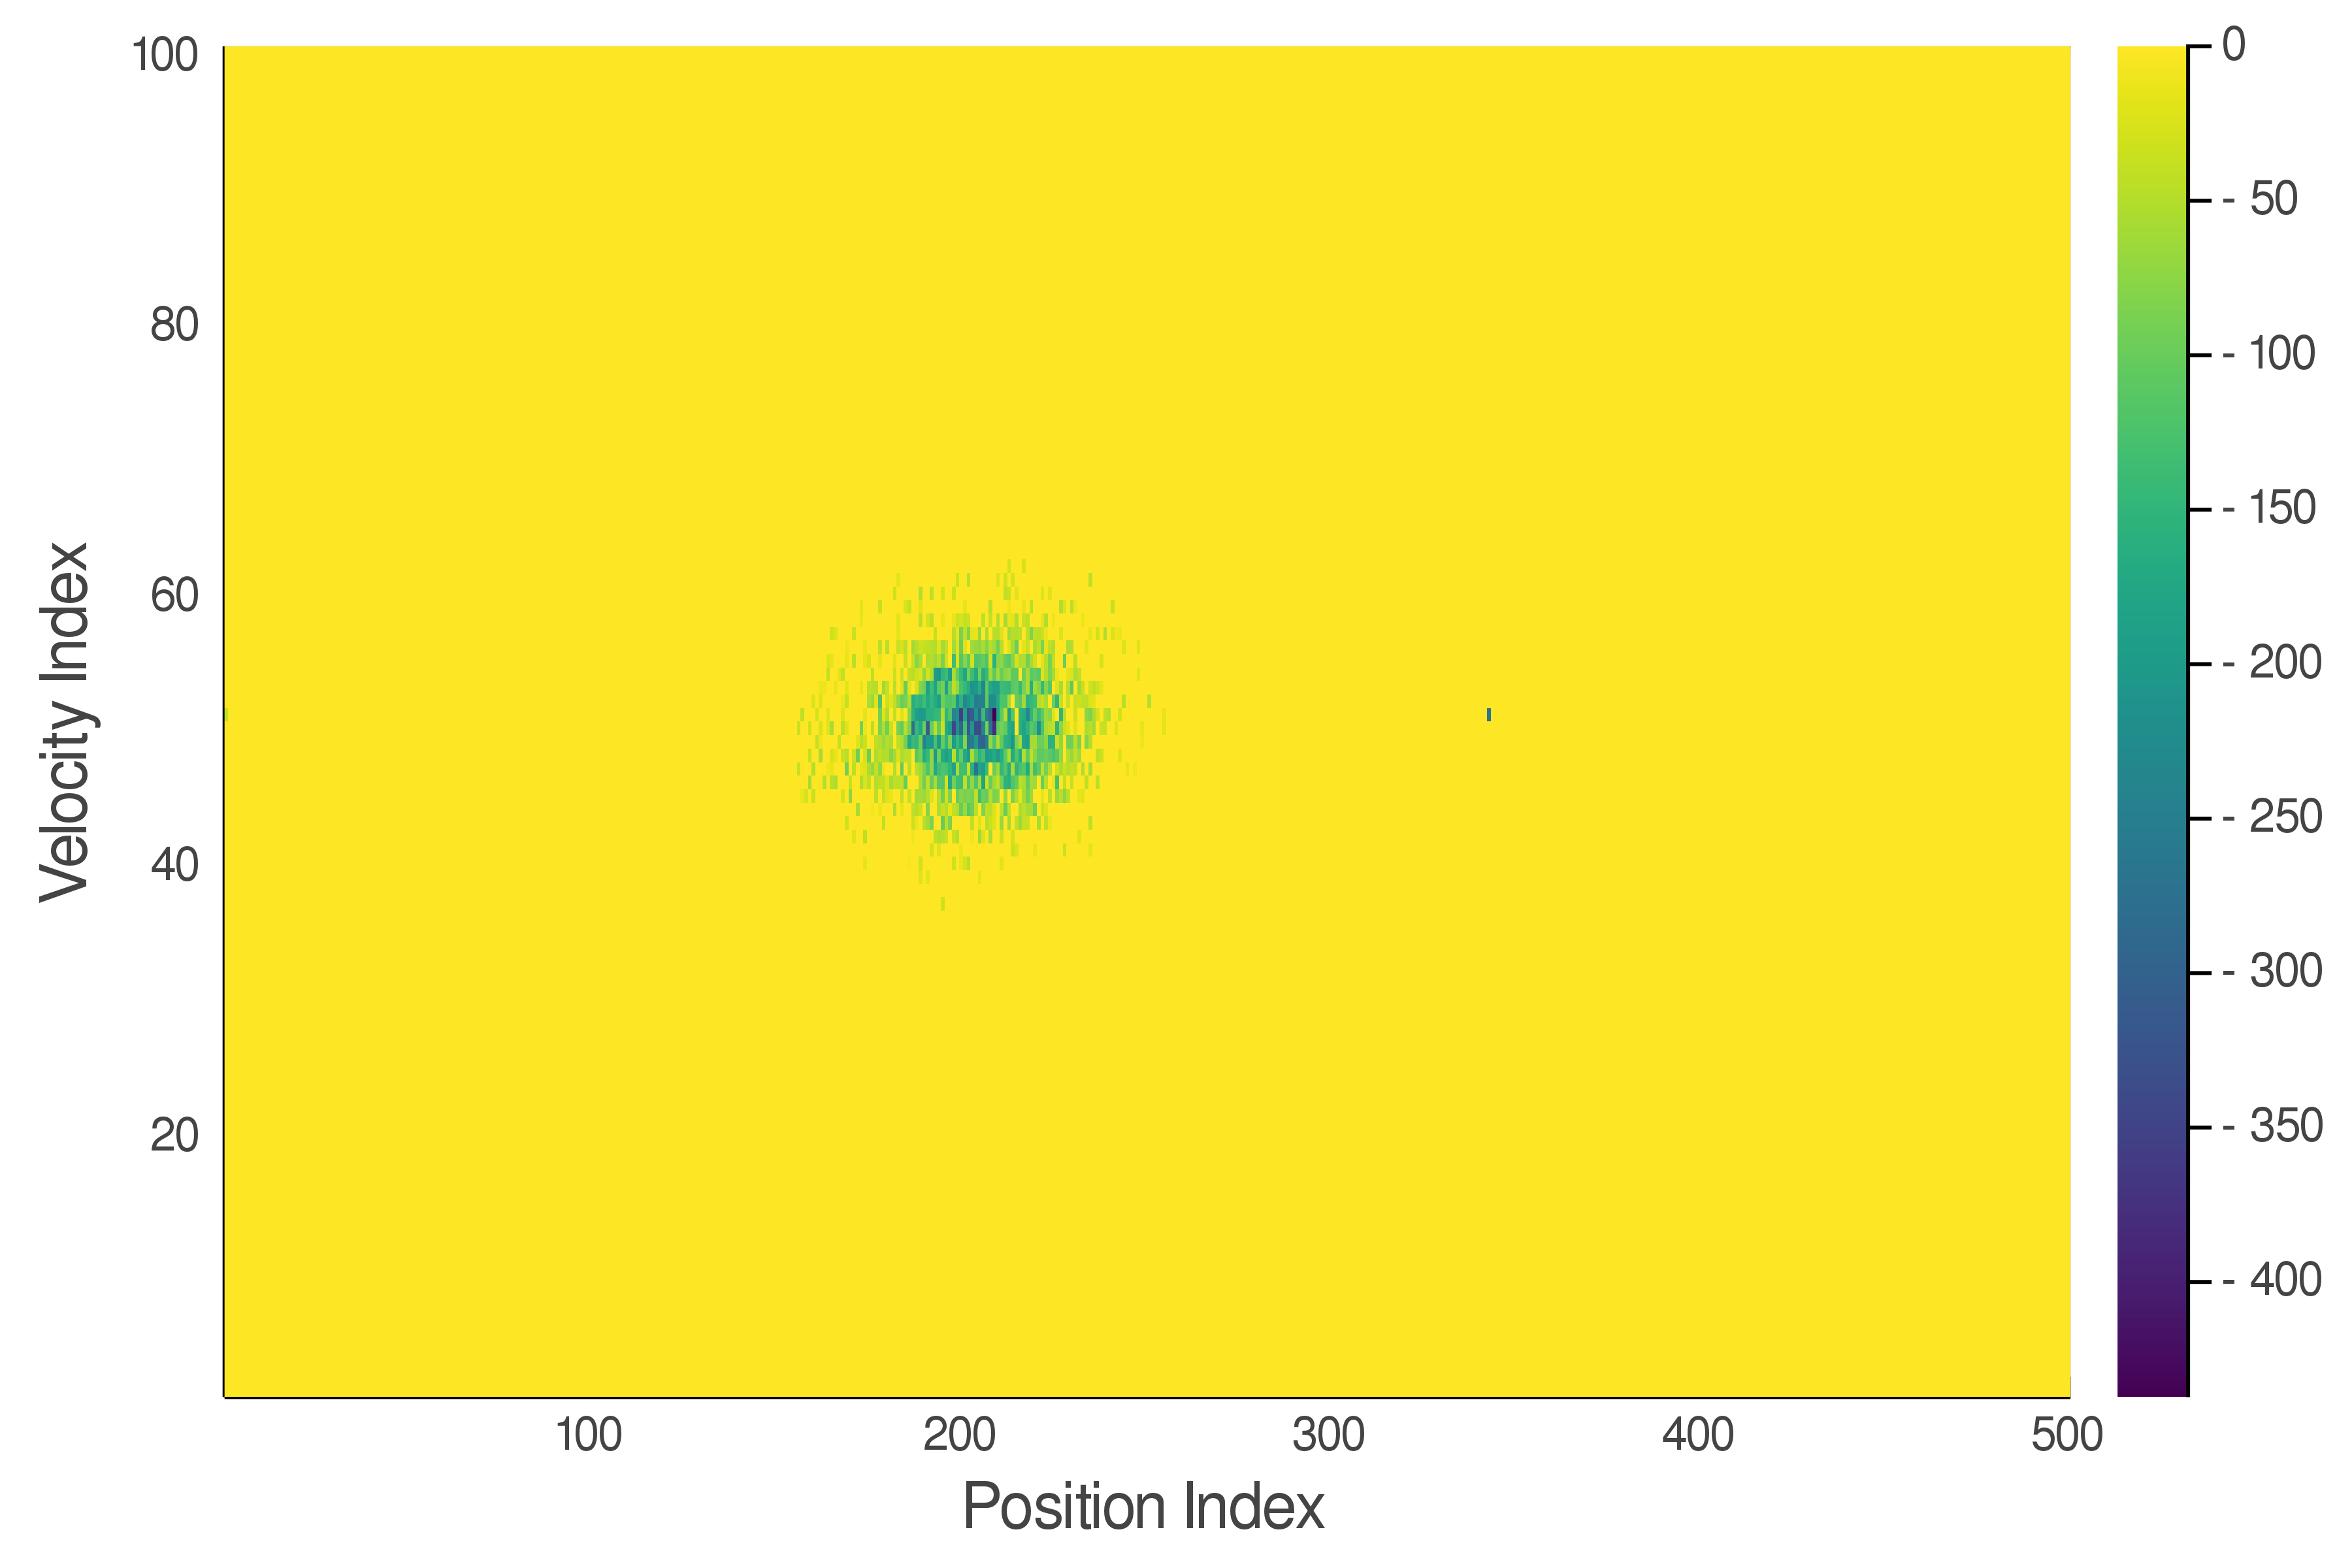
\includegraphics[width=\linewidth]{../plots/medium_U_sarsaLambda.png}
		\includegraphics[width=\linewidth]{../plots/medium_π_sarsaLambda.png}
		\captionof{figure}{Optimal value function and policy in the phase space representation using sarsa($\lambda$) ($\gamma = 0.99; \lambda = 0.9; \alpha = 0.05$) for the \texttt{medium} dataset.}
		\label{fig:medium_U_sl}
	\end{Figure}	
	\subsubsection*{\sf \textbf{Large Dataset}}
	The \texttt{large} dataset describes an unknown environment with $|\mathcal{S}| = 312020$ and $|\mathcal{A}| = 9$. The discount factor for the problem is given to be $\gamma = 0.95$. The dataset appears to have a convenient representation as three sets of coordinates ($ceil(s/10000), mod(s, 10000), mod(s, 100))$.
	We used only Gauss-Seidel value iteration to find an approximately optimal policy. The representation shown below is the compressed representation with the first coordinate along the y-axis, and the second coordinate along the x-axis (which is a composition of only the unique second coordinates, implying periodicity over the third coordinate). The challenge in this dataset is that the state space is quite large and so an efficient representation is needed to achieve a fast algorithm. Since we can only iterate on the states in our dataset, we have a reasonable compression of the state space itself, so the algorithm is faster that in the \texttt{medium} dataset despite the increased size of the state space and action space.
	\begin{Figure}
		\centering
		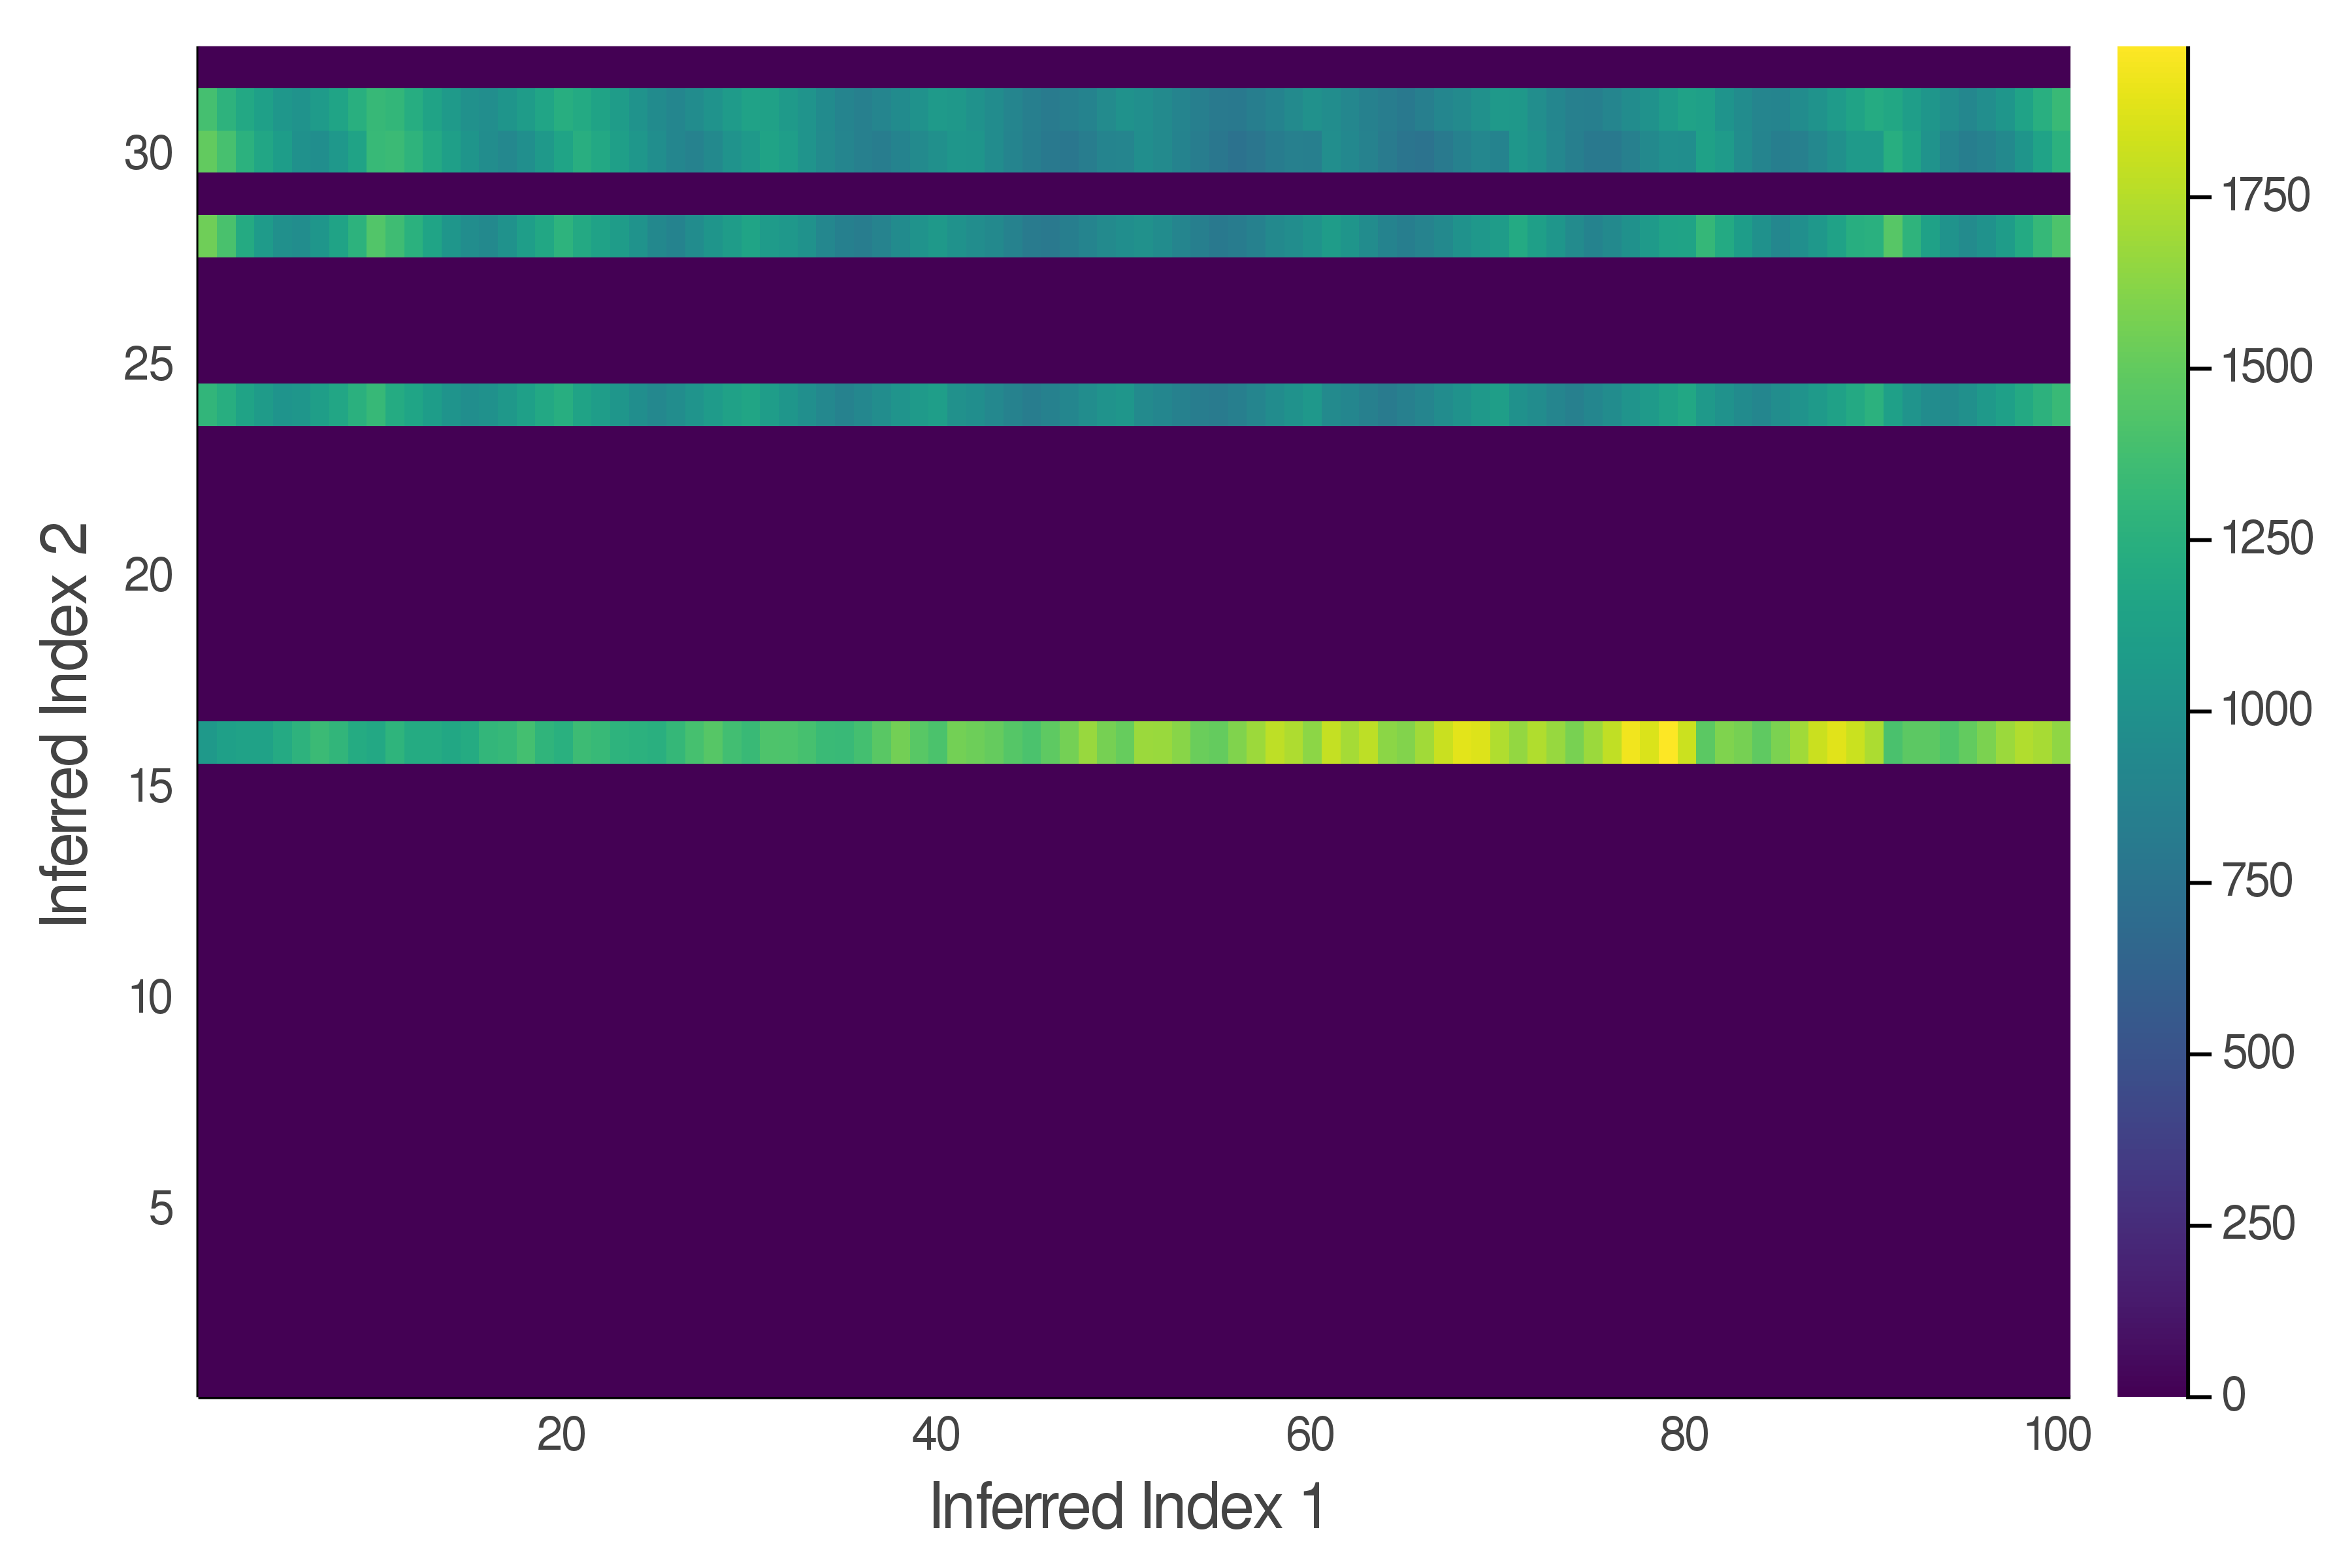
\includegraphics[width=\linewidth]{../plots/large_U_GSVI.png}
		\includegraphics[width=\linewidth]{../plots/large_π_GSVI.png}
		\captionof{figure}{Optimal value function and policy in the compressed representation using Gauss-Seidel value iteration ($\gamma = 0.95; \epsilon = 0.1$) for the \texttt{large} dataset.}
		\label{fig:large_U_GSVI}
	\end{Figure} \vspace*{-0.1 in}
	\begin{center}
		\captionof{table}{Runtimes in Seconds for Various Algorithms}
		\vspace*{10pt}
		\label{tab:runtime}
		\begin{tabular}{l|c|c|c|}
			\cline{2-4}
			                                       &                           \multicolumn{3}{c|}{\textbf{Algorithm}}                           \\ \hline
			\multicolumn{1}{|l|}{\textbf{Dataset}} & \multicolumn{1}{c|}{VI} & \multicolumn{1}{c|}{GSVI} & \multicolumn{1}{c|}{Sarsa($\lambda$)} \\ \hline
			\multicolumn{1}{|l|}{\texttt{small}}            & 1.264                   & 0.922                     & 1.046                                 \\ \hline
			\multicolumn{1}{|l|}{\texttt{medium}}           & -                       & 5460                      & 628.9                                 \\ \hline
			\multicolumn{1}{|l|}{\texttt{large}}            & -                       & 220.4                     & -                                     \\ \hline
		\end{tabular}
	\end{center}
	
\end{multicols*}
	
\end{document}